%!TEX root = main.tex
%!TEX encoding = UTF-8 Unicode

\chapter{Resources}
\label{chap:resources}

\lettrine{A} resource is an object used to protect a critical section in a task or in an ISR and to insure mutual exclusion.
By using a resource to protect the use of a shared piece of data or a shared hardware device, the programmer avoids race conditions.
Figure \ref{fig:exampleRaceCondition} shows an example of race condition.


\begin{figure}[htbp] %  figure placement: here, top, bottom, or page
   \centering
   \begin{minipage}[c]{.55\linewidth}
\begin{lstlisting}[language=C]
int val = 0;
int actCount = 0;

TASK(bgTask)
{
  while (1) {
    val++;
    val--;
  }
}

TASK(periodicTask)
{

  activationCount++;
  if ((actCount % 2) == 1) {
    val++;
  }
  else {
    val--;
  }
    
  TerminateTask();
}

TASK(displayTask)
{
  printf("val=%d count=%d\n",
         val,
         activationCount);
    
  TerminateTask();
}
\end{lstlisting}
   \end{minipage}\hfill
   \begin{minipage}[c]{.35\linewidth}
\begin{lstlisting}[language=C]
val=2 count=10
val=3 count=20
val=4 count=30
val=5 count=40
val=2 count=50
val=2 count=60
val=0 count=70
val=-2 count=80
val=-1 count=90
val=-1 count=100
val=-2 count=110
val=0 count=120
val=0 count=130
val=0 count=140
val=0 count=150
val=-2 count=160
val=-1 count=170
val=-2 count=180
val=-4 count=190
val=-4 count=200
val=-6 count=210
val=-4 count=220
val=-5 count=230
val=-6 count=240
val=-7 count=250
val=-6 count=260
val=-3 count=270
val=-3 count=280
val=-5 count=290
val=-5 count=300
\end{lstlisting}
   \end{minipage}
   \caption{{\bfseries Shared data access.} In this example 3 preemptable tasks are used. \constant{bgTask} increments and decrements the global integer variable \var{shared} in an infinite loop. \constant{periodicTask} runs every 100ms and increments the global integer variable \var{activateCount}. If \var{activateCount} is odd, \constant{periodicTask} increments \var{shared} otherwise it is decremented. A third task, \constant{displayTask} runs every second and displays both variables. On the left, the corresponding program, on the right one of the possible outputs}
   \label{fig:exampleRaceCondition}
\end{figure}

\section{\osek\ Priority Ceiling Protocol}

\osek\ uses a modified version of the Priority Ceiling Protocol\,\cite{PCP}. A priority is assigned to each resource. This 
priority is computed to be at least equal to the highest priority of the tasks and ISRs that use the resource. So let $T_1, T_2, \dots, T_n$ a set of tasks sharing the same resource $R$ and $P_1, P_2, \dots, P_n$ their priorities so that $P_i = P(T_i)$. We have $P(R) = \max_{i=1,n}(P_i)$.

When a task gets a resource, its priority is raised to the priority of the resource. That way, the task will run with the priority of the highest priority task and will insure the release of the resource is not delayed by a lower priority task. In addition, since every other tasks that use the same resource have now a priority $\leq$, they cannot preempt the running task and mutual exclusion is insured. Figure \ref{fig:exampleResource} show an example of resource use.

\begin{figure}[htbp] %  figure placement: here, top, bottom, or page
   \centering
   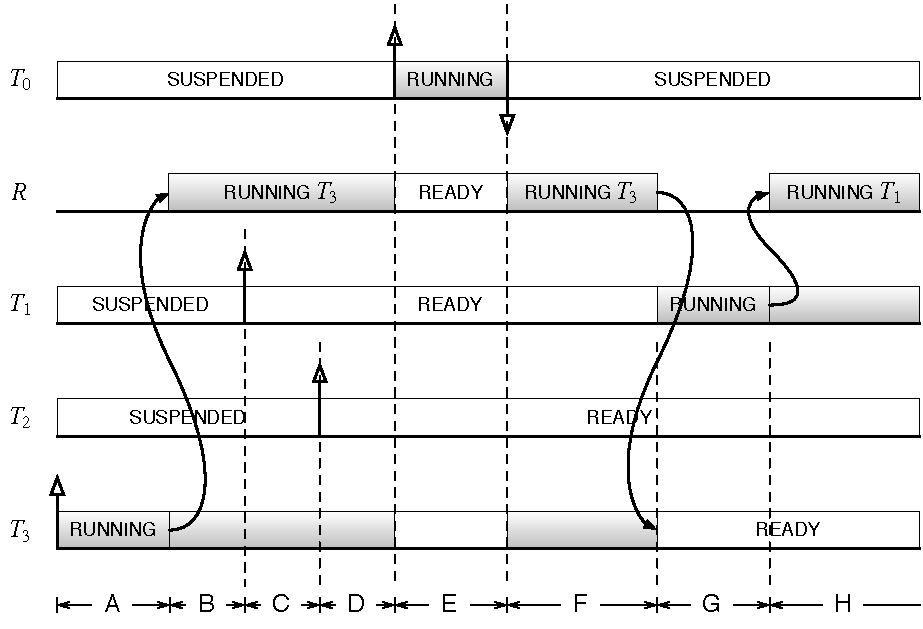
\includegraphics[scale=.7]{pictures/schedulingResource.pdf} 
   \caption{{\bfseries Scheduling with a resource used by 3 tasks and a fourth task having a higher priority.} $P(T_0)>P(T_1)>P(T_2)>P(T_3)$. $R$ is used by $T_1$, $T_2$ and $T_3$ so $P(T_0)>P(R)\ge P(T_1)$. During A period, $T_3$ is {\sffamily\scshape running} and other tasks are {\sffamily\scshape suspended}. Then $T_3$ gets $R$ and $P(T_3) \leftarrow P(R)$ (B to F periods). $T_1$ is activated and becomes {\sffamily\scshape ready}; since $P(T_3) \ge P(T_1)$, $T_1$ does not run (C to F periods). $T_2$ is activated and becomes {\sffamily\scshape ready}; for the same reason it does not run (D to H periods). $T_0$ is activated and because $P(T_0)>P(R)$ it runs (E period). $T_0$ terminates and $T_3$ continues its execution (F period). Then $T_3$ releases $R$ and $P(T_3)$ reverts to its base priority; so since $P(T_1)>P(T_2)>P(T_3)$, $T_1$ runs (G period). $T_1$ gets $R$ and $P(T_1) \leftarrow P(R)$ (H period).}
   \label{fig:exampleResource}
\end{figure} 

The priority of a resource is computed by \goil\ according to the priorities of the tasks and ISRs that use the resource.

\section{The {\normalsize RES_SCHEDULER} resource}

Trampoline provides a predefined standard resource called \constant{RES_SCHEDULER}. This resource has a priority $\ge$ to the maximum priority of the tasks but $<$ to the minimum priority of the ISR. When a task gets \constant{RES_SCHEDULER}, it becomes non preemptable. To make \constant{RES_SCHEDULER} available to the application, the \oilattr{USERESCHEDULER} attribute must be set to \TRUE\ within the \oilattr{OS} object in the OIL file. Unlike resources defined by the application, there is no need to declare \constant{RES_SCHEDULER} is used by a task in the OIL file.

\section{Standard and Internal Resources}

Standard resources are got and released explicitly by tasks and ISRs using the ad-hoc services. Internal resources are got implicitly when the task enters the \RUNNING\ state and released implicitly when the task calls \api{Schedule} or blocks when using \api{WaitEvent}.

\note{At most one internal resource may be used by a task.}

Standard resources are dedicated to the protection of critical sections around the access to a shared data or to a device. Internal resources are used to implement non preemptable tasks within a task group.
A task group is a set of task that are non preemptable by each other but remain preemptable by higher priority tasks in the application. A task group priority is the priority of its internal resource.

Trampoline provides a predefined internal \constant{RES_SCHEDULER} resource with the same priority. This internal resource is used to implement non preemptable tasks in the whole application as if all the non preemptable tasks belong to an implicit task group. When a task is non preemptable by setting the \oilattr{SCHEDULE} attribute to \constant{NON} in its OIL description, the task is assigned the internal \constant{RES_SCHEDULER} resource.

\section{Nested resources accesses}
\label{sec:resnested}

Resources may be accessed in a nested way. That is once a resource is got, another one may be got before releasing the first one and so on. However resources must be released in the reverse order they have been got as if they were pushed on a stack. The following example shows the good usage of resources:

\begin{lstlisting}
TASK(MyTask)
{
  GetResource(rez1);
  ...
  /* critical section protected by rez1 */
  ...
  GetResource(rez2);
  ...
  /* critical section protected by rez2 and rez1 */
  ...
  ReleseResource(rez2);
  ...
  /* more critical section protected by rez1 */
  ...
  ReleaseResource(rez1);
  TerminateTask();
}
\end{lstlisting}



\section{OIL description}

A resource is described using a \oilattr{RESOURCE} object. \oilattr{RESOURCEPROPERTY} is the single attribute of this object. A standard resource is defined with the following code:

\begin{lstlisting}[language=OIL]
RESOURCE res {
  RESOURCEPROPERTY = STANDARD;
};
\end{lstlisting}

And an internal resource is defined with the following code:

\begin{lstlisting}[language=OIL]
RESOURCE other_res {
  RESOURCEPROPERTY = INTERNAL;
};
\end{lstlisting}

A third kind of declaration exists for {\bfseries\oilattr{LINKED}} resources. A linked resource may be linked to a linked resource or a standard resource but a link tree of resources must have a standard resource at the root. A linked resource has the same priority as the standard resource it is linked to and is a kind of reference. Linked resources are provided to replace nested access to the same resource (which is prohibited) and are rarely used.

\begin{lstlisting}[language=OIL]
RESOURCE l_res {
  RESOURCEPROPERTY = LINKED { LINKEDRESOURCE = res };
};
\end{lstlisting}

\warning{Every task and ISR that uses a resource in the C code must declare it in the OIL file. Otherwise \goil\ will compute a wrong priority for the resource and the scheduling of tasks and the execution of ISR will not be as expected.}

\section{Resources services}

\begin{service}{DeclareResource}{}
\argument{ResourceType}{ResourceID}{The id of the resource}
Each resource has an identifier of type \ctype{ResourceType}. This identifier is declared in the OIL file and is used in system calls to refer to a particular resource. \servicename\ declares a resource exists. The result is to make the id of the resource available and allows to use it in services' calls.

\note{\servicename\ is a C macro}
\end{service}

\begin{service}{GetResource}{StatusType}
\argument{ResourceType}{ResourceID}{The id of the resource to get}
\servicename\ enters the critical section protected by the resource. For each call to \servicename, a corresponding call to \api{ReleaseResource} must be made in the control flow of the task or ISR. Nested calls are allowed, see \ref{sec:resnested} for nested resource accesses.
\resultcode{\OK}{No error}
\resultcode{\OSID}{Invalide resource id. No resource with such an id exists}
\resultcodeext{\OSACCESS}{The resource is already taken by a task or an ISR or has a priority lower than the base priority of the calling task or ISR. This should not happen if the application is configured correctly except if the same task or ISR try to get the same resource twice}
\end{service}

\begin{service}{ReleaseResource}{StatusType}
\argument{ResourceType}{ResourceID}{the id of the resource}
\servicename\ leaves the critical section protected by the resource. For each call to \servicename, a corresponding call to \api{GetResource} must have been made in the control flow of the task or ISR. Nested calls are allowed, see \ref{sec:resnested} for nested resource accesses.

\note{This service does a rescheduling}

\resultcode{\OK}{No error}
\resultcode{\OSID}{Invalide resource id. No resource with such an id exists}

\end{service}